\chapter{Vorbetrachtungen}
\section{Client-Server Architektur}
Die Basis für die meisten Anwendungen im Web bildet die Client-Server Architektur.
Der Nachrichtenaustausch in einem verteilten System wird dabei auf zwei Akteure und eine Interaktion fokussiert.
Der Client initiiert die Interaktion, indem er eine Nachricht an den Server sendet.
Der Server reagiert, indem er mit dem Resultat der Auswertung der Nachricht antwortet.
Ein Client kann mit mehreren Servern in Interaktion treten und mehrere Clients können mit dem gleichen Server kommunizieren, wie in Abbildung~\ref{img:client-server} dargestellt.
Durch die Anfrage werden die Rollen von Client und Server festgelegt, welche jedoch nur für die Dauer der Interaktion gelten.
So kann ein Akteur, der bei einem Nachrichtenaustausch als Server angefragt wird, während eines anderen selbst als Client die Kommunikation beginnen.
Bedingungen für die Client-Server Architektur sind, dass dem Client zu Beginn der Kommunikation der Server bekannt ist und dass beide das gleiche Kommunikationsprotokoll unterstützen.
\begin{figure}[h]
  \centering
  \fbox{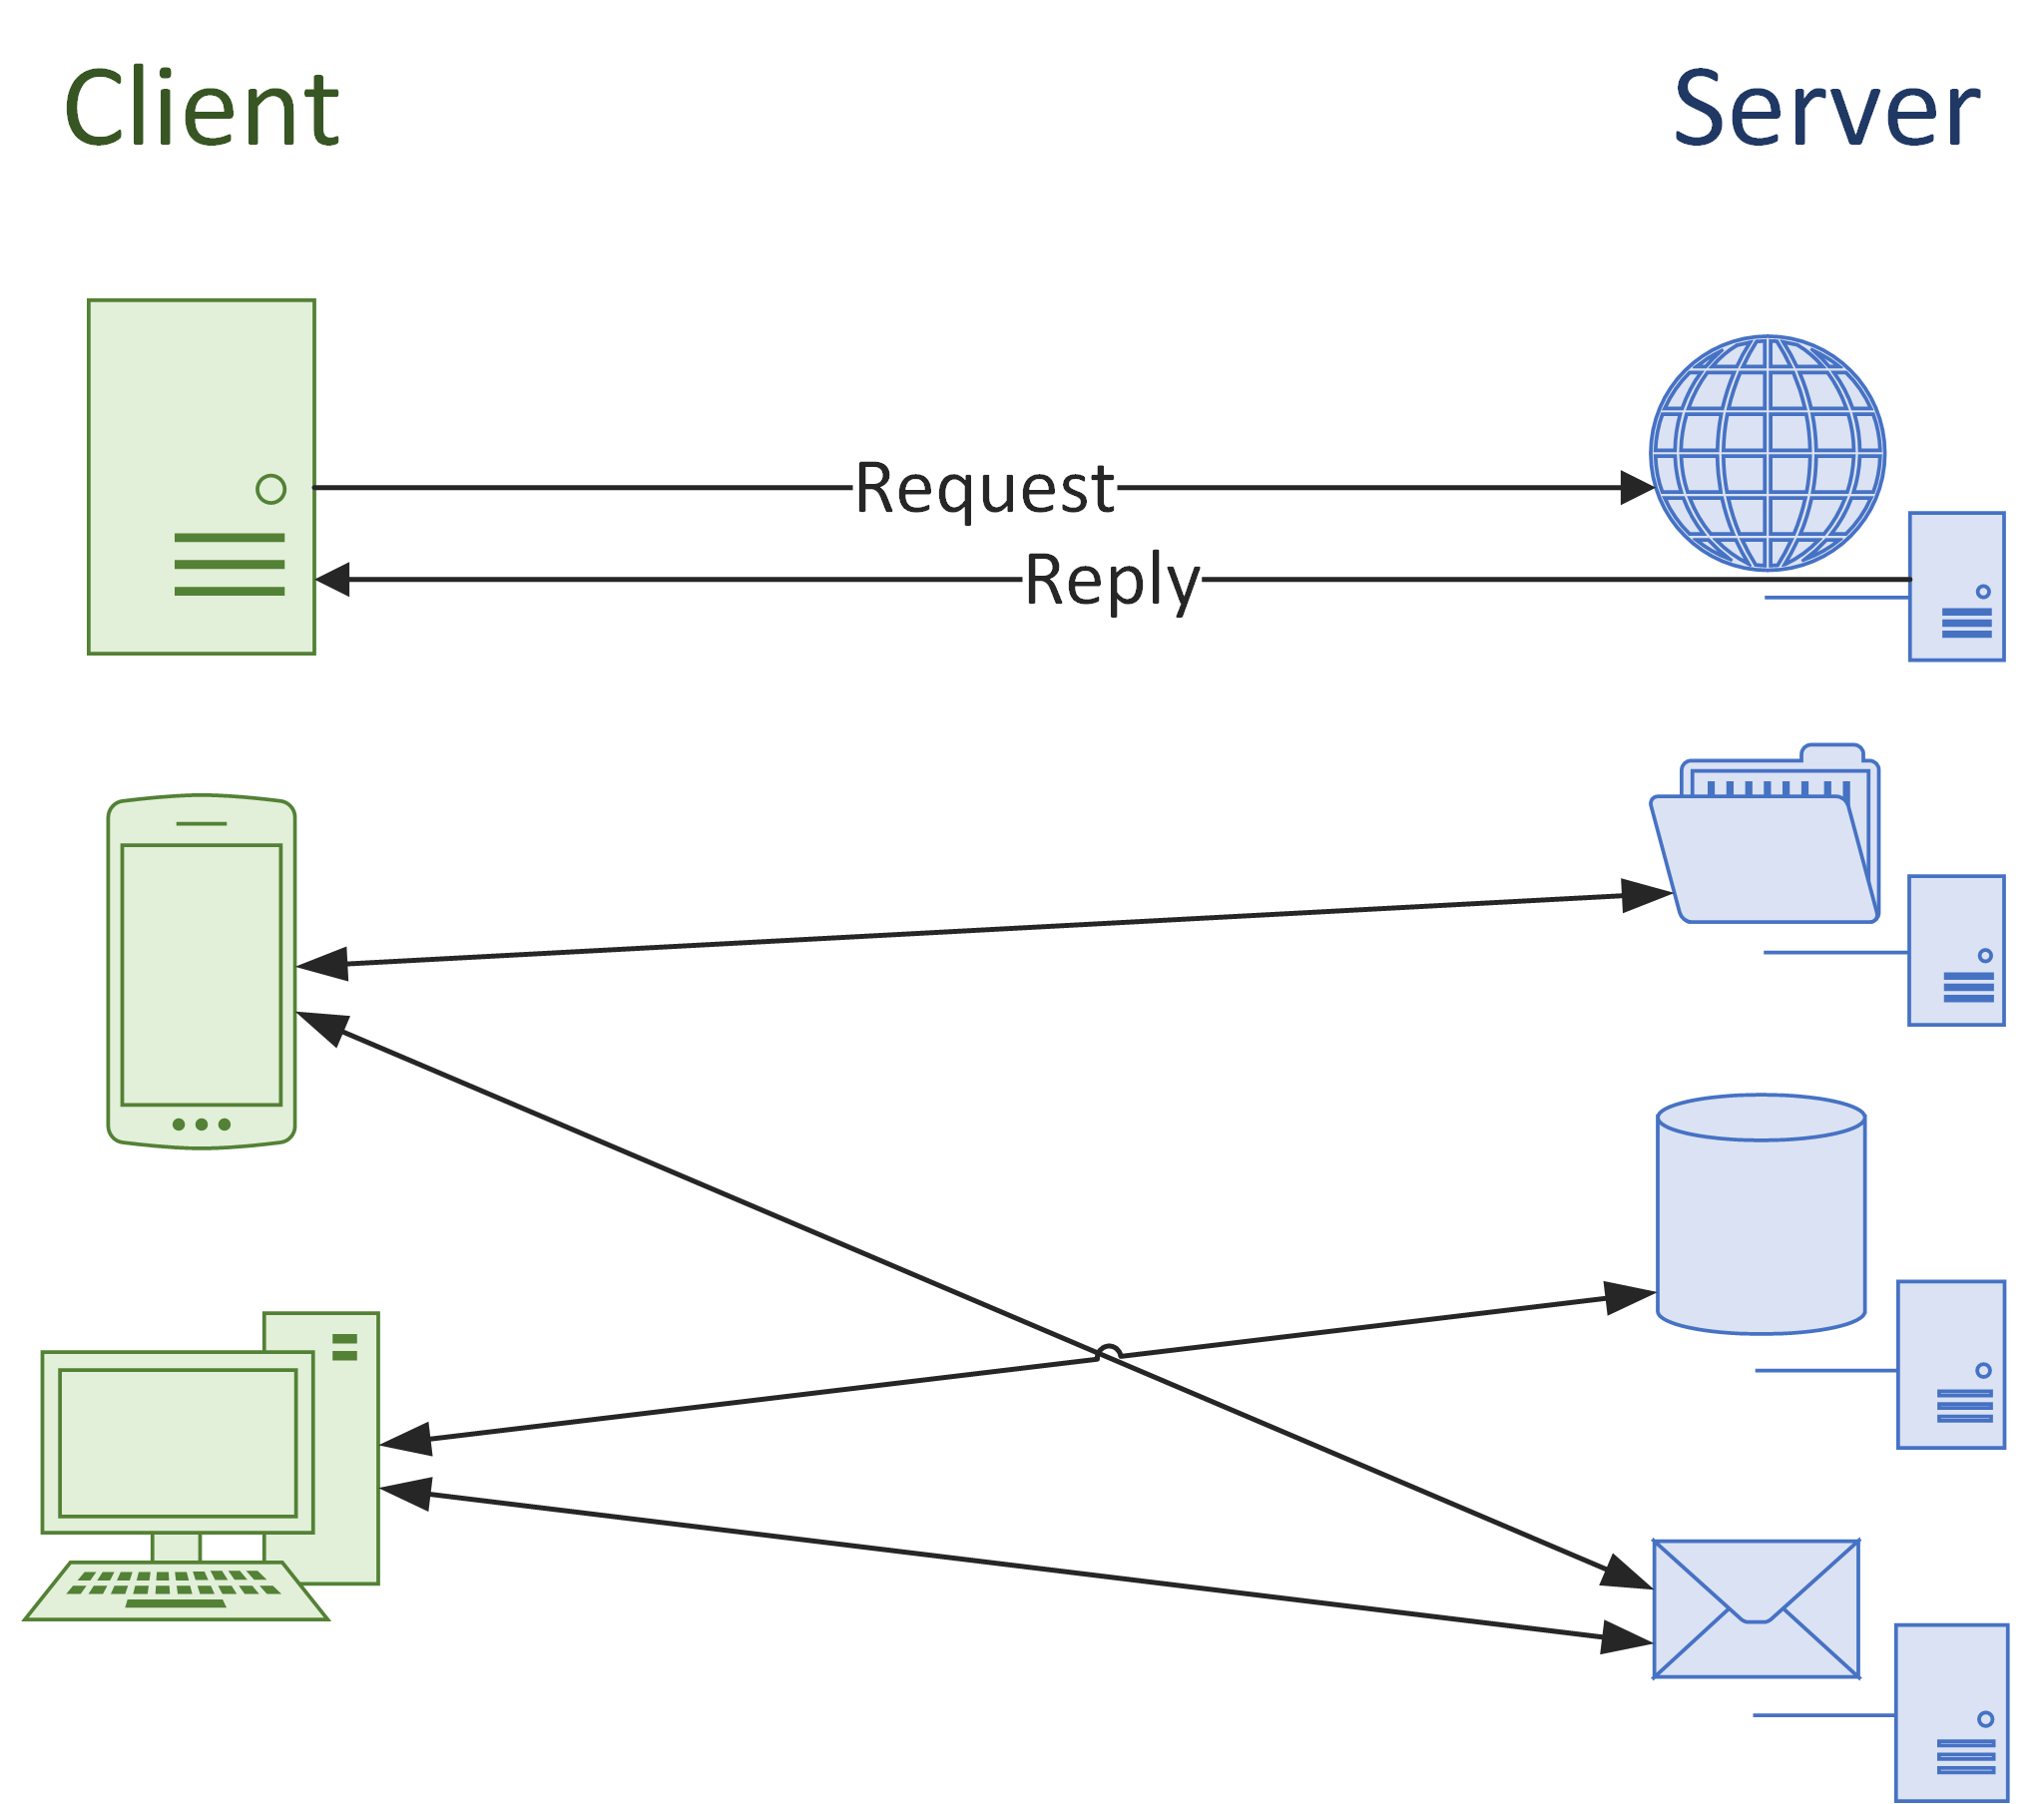
\includegraphics[width=10cm]{client-server.png}}
  \caption{Mehrere Clients treten mit verschiedenen Servertypen in Interaktion, in Anlehnung an~\cite[23]{Bengel}}\label{img:client-server}
\end{figure}
\par
Die Entwicklung einer Anwendung nach dieser Architektur hat ein erklärtes Ziel und Hauptvorteil: Die Trennung der Verantwortlichkeiten.\cite[vgl.][78]{REST}
\par
Client und Server sind logisch und oft auch physikalisch getrennte Teile einer Anwendung und können unabhängig voneinander entwickelt werden, solange sie ihre Kommunikationsschnittstelle wahren.
Die damit verbundene Trennung der Verantwortlichkeiten führt zu einer Reduzierung der Komplexität der einzelnen Anwendungsteile.
Da Client und Server unabhängig voneinander ausgeführt werden, beeinflusst der Ausfall des einen nicht die Stabilität des anderen.
Wird der Client als Benutzeroberfläche und der Server als Datenspeicher genutzt, so können beispielsweise mehrere Clients für verschiedene Geräte oder Anwendungsfälle entwickelt und optimiert werden, wodurch die Portabilität der Oberfläche verbessert wird.
Die Verteilung auf mehrere Geräte erhöht außerdem die Skalierbarkeit des Gesamtsystems.

\section{Web APIs}
Eine Software kann einen Teil seiner Funktionalität über Schnittstellen externen Programmen zur Verfügung stellen.
Solche Application Programming Interfaces (API) ermöglichen die Kommunikation zwischen Programmen durch das parametrisierte Aufrufen der öffentlich gemachten Funktionen einerseits und das Antworten mit dem Ergebnis der Funktion andererseits.
Ein großer Vorteil der Verwendung von APIs ist das Verstecken der zugrundeliegenden Komplexität und führt zu Unabhängigkeit von Implementierungsdetails.
So ist es z.B.\ die Aufgabe eines Betriebssystems, Programmen den Zugriff auf Hardwarekomponenten, wie Dateisystem, Netzwerk, Sensoren und Peripheriegeräte, zu abstrahieren und bereitzustellen.
Externe Programme werden durch die Benutzung jedoch abhängig von der Schnittstelle, welche daher als Kommunikationsobjekt Vertragscharakter bekommt.
Für die meisten Programmiersprachen existieren Programmbibliotheken und Frameworks, die zur Entwicklungszeit grundlegende und immer wieder benötigte Funktionalität bereitstellen, aber besonders Cloudservices und öffentliche APIs haben in den letzten Jahren an Popularität erlangt, da sie mit HTTP eine sprachunabhängige Schnittstelle bieten und die Integration von Anwendungs- und Nutzerdaten ermöglichen.
Die vorliegende Arbeit beschränkt sich auf API von verteilten Systemen im Web.
Webanwendungen auf Basis von JavaScript-Frameworks werden häufig auch als Fat-Client Anwendungen bezeichnet, da ein beträchtlicher Teil der Programmlogik, sowie die Benutzeroberfläche auf Clientseite ausgeführt wird.
Da der Server in solchen Anwendungen als Zugangspunkt und Speicher für Daten dient, sind die APIs geprägt von der Übertragung der Daten zur Anzeige im Client und der Modifikation der Daten auf dem Server.
Gemäß den Hauptinteraktionen werden diese APIs auch als CRUD (Create, Read, Update, Delete) APIs bezeichnet.
\subsubsection{Abgrenzung zu anderen Web API Ansätzen}
Neben REST und GraphQL existieren weitere API-Technologien auf Basis der Client-Server-Architektur wie das Simple Object Access Protocol (SOAP) und Remote Procedure Call (RPC).
SOAP verwendet XML zur Kommunikation, welches an vielen Stellen durch das leichtgewichtigere JSON abgelöst wurde.
Ziel einer RPC-Kommunikation ist das Aufrufen einer Aktion auf dem Server, wobei die Orientierung an Funktionsnamen zu einer engen Kopplung von Client und Server führt.
Die Namensgebung der Funktionen erfordert außerdem Dokumentation und Richtlinien, um einen Überblick über bestehende Funktionen zu erhalten und die Zahl derselben nicht unnötig zu vergrößern und damit die Komplexität der API zu erhöhen.
RPC ist aufgrund seiner leichtgewichtigen Nachrichten für Anwendungen mit hohen Performanceansprüchen oder befehlorientierte APIs geeignet~\cite[vgl.]{Barbettini}.
Beide Technologien finden jedoch in der Entwicklung von Single-Page-Apps kaum Verwendung und sollen daher im Folgenden nicht weiter betrachtet werden.
